\documentclass[12pt]{article}
\usepackage[margin=2.5cm]{geometry}
\usepackage{multicol}

\usepackage{url}
\usepackage{graphicx}
\usepackage{amsmath}
\usepackage{epsfig}
\usepackage{color}
\usepackage{amssymb}
\usepackage{amsfonts}
\usepackage{setspace}
\usepackage{subfigure}
\usepackage{soul}
\usepackage{mathrsfs,amsmath}

\begin{document}
\color{black}
\begin{center}\textbf{\large CSC413 Project Proposal}\\\bigskip

 {\bf Abhijoy Mandal; 1005714121
  }
\end{center}

\noindent

\section{Introduction}

Deep generative models have seen a huge leap in popularity in recent years, particularly in high fidelity text-to-image generation ~\cite{ramesh2021zeroshot}. This has been facilitated mostly by diffusion models, which posses stable and scalable ways to train them ~\cite{NEURIPS2020_4c5bcfec}. These models however move through complicated probability paths during denoising, resulting in longer training and inference times. ~\cite{lipman2023flow}
\\
Continuous Normalizing Flows provide a way to model arbitrary probability paths, and recent advances in this line of work has led to the development of tractable and differentiable ways to train CNF based models. These models have shown the ability to outperform DDPM based models both in terms of quality of images (measure by FID) and in terms of speed of inference (measured by NFE) ~\cite{lipman2023flow}. While CNF models show impressive performance in unconditioned image sampling, their capabilities text conditioned sampling remains unexplored.
\\
In this project, we look to explore the possibility of conditioning flow matching models on text prompts as well as explore the zero-shot generation capabilities of such models.

\section{Prior Works}
\subsection{Zero-shot Text-to-Image}
The problem of zero-shot text-to-image generation deals with generating high-fidelity images conditioned on text prompts, possibly unseen by the model. Diffusion models have shown impressive performance at this task outperfoming SOTA GAN models at generating realistic images, achieved by training on much larger datasets (such as LIAON-5B ~\cite{schuhmann2022laion}) consisting of image text pairs ~\cite{ramesh2021zeroshot, saharia2022photorealistic}. Following the initial success of diffusion models, several improvements had been made to reduce model size (latent diffusion ~\cite{rombach2022high}), improve image quality (cascaded diffusion ~\cite{ho2022cascaded}) and increase the modality of outputs (using VAE ~\cite{ramesh2021zeroshot}). All these methods, however, use diffusion models and CNFs remain largely unexplored in this field which provide an opportunity to further improve on existing architectures both in terms of speed and quality of images.

\subsection{Generative Flow Matching}
Flow matching algorithm follows from Continuous Normalising Flows, which aim to model the movement of the probability distribution (probability paths) by predicting vector fields which dictate how to move the probability distribution from an initial prior (say random noise) to a distribution on interest (say an image).  However until late, most methods of training such models required expensive simulations of ODEs or involved intractable calculations hindering widespread use. Recent works in this field address this and have successfully managed to train flow mathcing networks for generative modelling, and have shown to outperform SOTA diffusion models in both quality and speed. The main set of reasons proposed for this improvement is that the flow matching vector fields are easier to model using neural networks and the probability paths to denoise an image are direct and have constant velocities making inference faster. ~\cite{lipman2023flow}

\section{Dataset and Model Architecture}
\begin{figure}[ht]
  \centering
  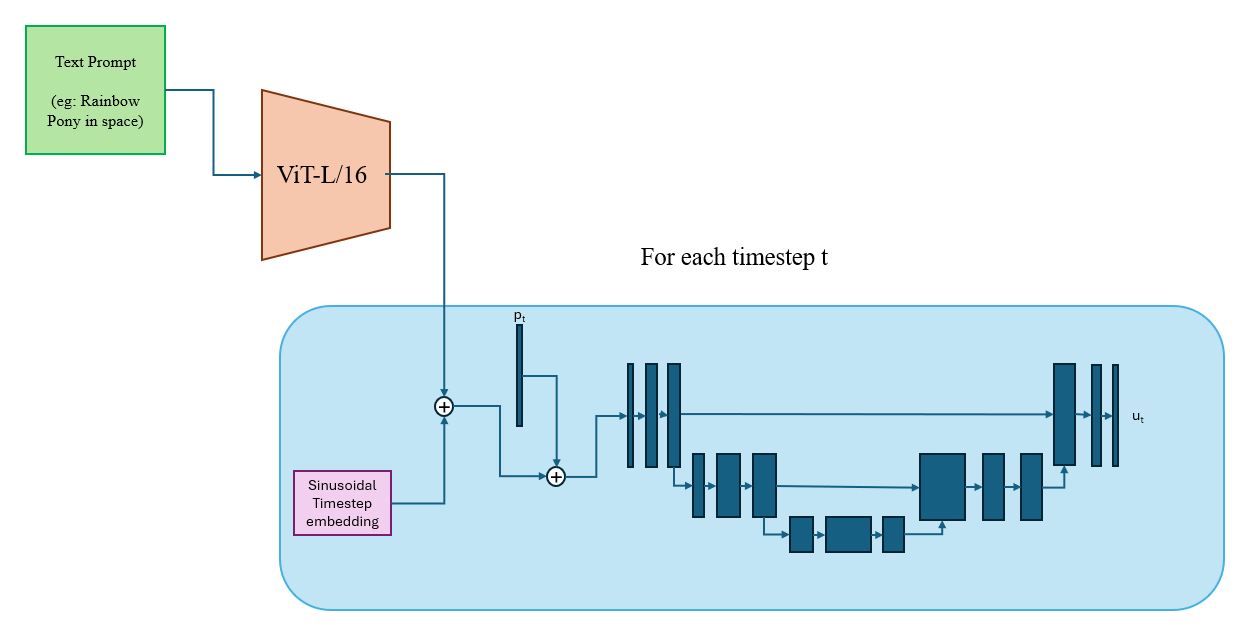
\includegraphics[width=0.75\linewidth]{Figures/model_arch.png}
  \caption{Model Architecture: At each timestep, we denoise the image $p_t$ conditioned on the sinusoidal timestep embedding and the text embedding, by adding these embeddings to $p_t$ and predict the vector field $u_t$, which is applied to $p_t$ using the push-forward function described in the flow matching paper. Note: we will use torchcfm, a package containing the mathematical utilities required to perform flow matching and their U-net architecture.}
\end{figure}
Large scale text-to-image models have been traditionally trained on large datasets consisting of image-text pairs. But these datasets tend to be several terabytes in size, making them unsuitable to be downloaded and used locally. Hence we look for datasets that can be streamed using WebDataset ~\cite{aizman2019high}, a dataset steaming pipeline made specifically for high performance I/O from remote datasets. In addition, we also need to ensure that datasets contain high quality text-to-image data, preferably with the dataset containing images rather than URLs to reduce training latency. We found datasets on HuggingFace that fit one or more of these criteria, for example LIAON-5B subsets and datasets similar to LAION-5B such as ``coyo-700m'', ``laion-coco-aesthetic'' and ``laion-coco-nllb'' (contain URLs making data streaming slow), artificially generated dataset such as ``diffusiondb'' (not in WebDataset format reducing streaming speed) and smaller datasets like COCO ``coco-karpathy''. However, we found one dataset that fit all these requirements, called, Conceptual 12M ``cc12m-wds'' ~\cite{changpinyo2021cc12m} which contains 12 million image-text pairs in WebDataset format, making it ideal for streaming.

The model consists of a text encoder and a flow matching U-net. We use a pre-trained CLIP ViT-16L as our text encoder as it is one of the more commonly used image-text models. The text-encoder is frozen during training as our main goal is to evaluate the use of flow matching instead of diffusion. Our goal is to successfully incorporate text embedding in flow matching, to achieve this, we explore with augmenting the timestep embeddings passed into the U-net with the text embedding obtained from a pre-trained ViT-16L. To reduce model size, we work in the 64x64 image space, but it is difficult to evaluate model performance on such low resolution images. To address this, we compare two approaches, one using off-the-shelf prompt-free superresolution models (because superresolution models tend to be diffusion models, and passing a text prompt makes it difficult to attribute  image generation quality to flow mathcing or diffusion part of the model) and the other where we train a superresolution model with a similar U-net structure.

Finally, we evaluate the zero-shot generation capabilities of flow matching based generative models by reporting FID and NFE statistics (to measure fidelity and speed) of these models on unseen text prompts, and compare these to SOTA diffusion policies.

\section{Compute resources}
Since we are training the model on a relatively small resolution and using a frozen, pre-trained text encoder, our model fits and is trainable on the free GPUs available on google colab. Further since we are streaming the datasets, we do not require any local storage, hence we plan to use the GPU compute on google colab to train our models.

\bibliography{Bibliography/Bibliography}
\bibliographystyle{IEEEtran}

\end{document}